% ============================================================
%  第 5 章  数值方法：有限差分与 SciPy 计算（扩展版）
% ============================================================

\chapter{数值方法：有限差分与 SciPy 计算}

\section{本章概览与学习路线}

前三章建立了物理问题的解析框架：分离变量、特殊函数、积分变换。但现实世界远比教科书复杂——非均匀介质、非线性项、不规则边界，这些都会使解析解遥不可及。

数值方法不是解析方法的替代，而是\textbf{互补}：
\begin{itemize}
\item 解析解提供物理洞察和参数标度律。
\item 数值解提供特定条件下的定量预言。
\end{itemize}

本章以\textbf{有限差分法} 为主线，结合 Python 的 NumPy/SciPy 生态，让你亲手"计算"前三章的偏微分方程。你将看到分离变量法给出的本征函数如何转化为矩阵本征值问题，傅里叶变换如何用 FFT 在 $O(N\log N)$ 时间内完成。

\begin{center}
\fbox{\parbox{0.9\textwidth}{\centering
\textbf{核心逻辑链条：}\\
连续 PDE $\to$ 网格离散 $\to$ 差分近似 $\to$ 稀疏矩阵 $\to$ 代数方程组求解
}}
\end{center}

\subsection*{不同读者的学习路径}

\begin{itemize}
\item \textbf{物理专业学生：} 重点关注 \S5.2--\S5.5（有限差分基础与 PDE 离散化），\S5.7（矩阵本征值问题——量子力学的数值视角），\S5.8（FFT 与谱方法）。
\item \textbf{计算科学学生：} 重点关注 \S5.2（截断误差与收敛性分析），\S5.3--\S5.5（不同时间步进格式的稳定性），\S5.10（误差分析与网格收敛性研究）。
\item \textbf{工程学生：} 重点关注 \S5.3--\S5.6（综合案例）中的可运行代码，直接应用于实际问题。
\end{itemize}

\section{有限差分基础}
\label{sec:fd_basics}

\subsection*{动机：计算机只能做加减乘除，如何让它求导？}

计算机不能理解 $\lim_{h\to 0}$，它只能计算加法、减法和乘法。有限差分的核心是放弃了"极限"，用一个小量 $h$ 来近似——这等价于把连续空间离散化为网格。放弃一定的精度换取可计算性，这就是数值分析的基本哲学。

\subsection{导数的差分近似}

由泰勒展开：
\begin{equation}
f(x+h) = f(x) + h f'(x) + \frac{h^2}{2}f''(x)
+ \frac{h^3}{6}f'''(x) + \cdots
\end{equation}

\textbf{一阶向前差分：}
\begin{equation}
f'(x) \approx \frac{f(x+h) - f(x)}{h},\quad \text{截断误差 } O(h).
\label{eq:forward_diff}
\end{equation}

\textbf{一阶向后差分：}
\begin{equation}
f'(x) \approx \frac{f(x) - f(x-h)}{h},\quad O(h).
\label{eq:backward_diff}
\end{equation}

\textbf{一阶中心差分：}
\begin{equation}
f'(x) \approx \frac{f(x+h) - f(x-h)}{2h},\quad O(h^2).
\label{eq:central_diff}
\end{equation}

\textbf{二阶中心差分：}
\begin{equation}
f''(x) \approx \frac{f(x+h) - 2f(x) + f(x-h)}{h^2},\quad O(h^2).
\label{eq:second_diff}
\end{equation}

\subsection{截断误差的详细推导}

以二阶中心差分为例，写出 $f(x\pm h)$ 的泰勒展开：
\begin{align}
f(x+h) &= f(x) + hf'(x) + \frac{h^2}{2}f''(x) + \frac{h^3}{6}f'''(x) + \frac{h^4}{24}f^{(4)}(x) + \cdots,\\
f(x-h) &= f(x) - hf'(x) + \frac{h^2}{2}f''(x) - \frac{h^3}{6}f'''(x) + \frac{h^4}{24}f^{(4)}(x) + \cdots.
\end{align}

两式相加，消去奇数阶导数项：
\begin{equation}
f(x+h) + f(x-h) = 2f(x) + h^2 f''(x) + \frac{h^4}{12}f^{(4)}(x) + O(h^6).
\end{equation}

整理得：
\begin{equation}
f''(x) = \frac{f(x+h) - 2f(x) + f(x-h)}{h^2} - \frac{h^2}{12}f^{(4)}(x) + O(h^4).
\end{equation}

因此截断误差的主项是 $-\frac{h^2}{12}f^{(4)}(x)$，阶数为 $O(h^2)$。

\begin{insight}
中心差分比单侧差分精度高一个阶次，因为对称性消去了 $O(h)$ 项。这如同量子力学中中心势 $V(-x)=V(x)$ 使波函数具有确定宇称——对称性在这里简化了问题并提高了精度。
\end{insight}

% 有限差分模板图
\begin{figure}[H]
\centering
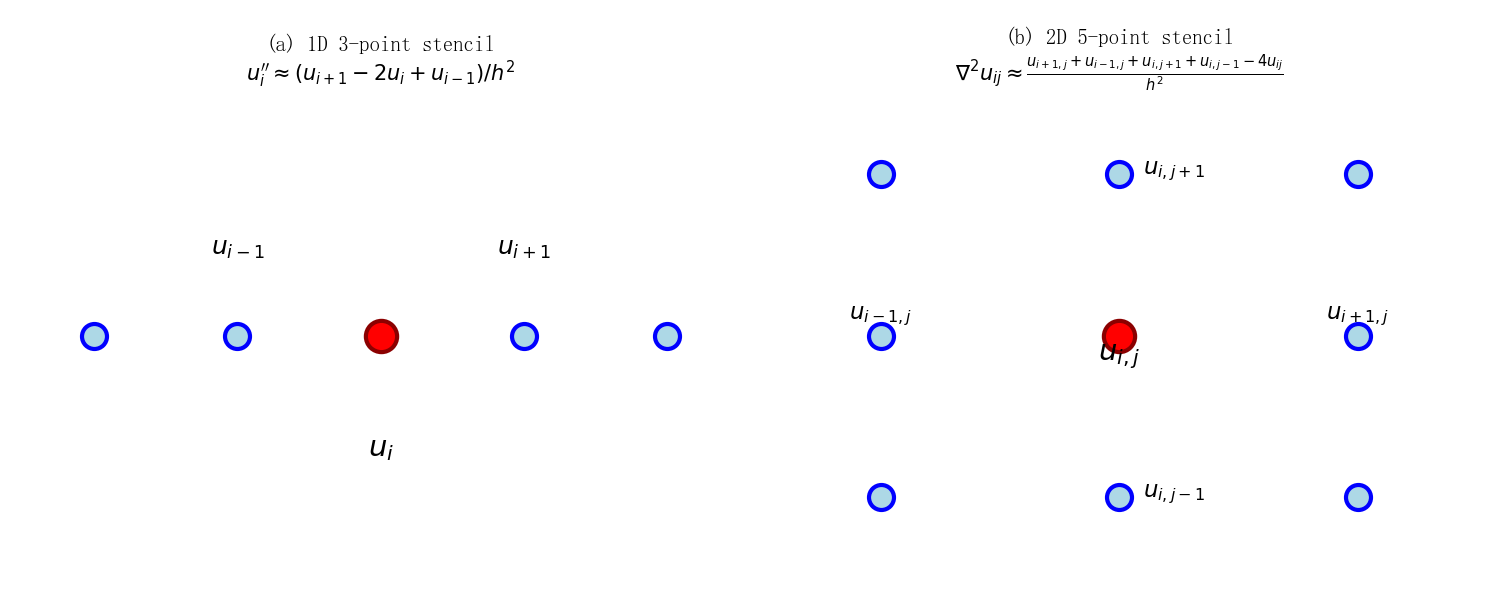
\includegraphics[width=0.8\textwidth]{figures/fig5_1_fd_stencil.png}
\caption{有限差分模板。左：一维三点模板，用于离散二阶导数。右：二维五点模板，用于离散拉普拉斯算子。红点为中心点 $u_{i,j}$，蓝点为邻点。}
\label{fig:fd_stencil}
\end{figure}

\subsection{差分模板与五点格式}

对于二维区域 $(x_i,y_j)$，拉普拉斯算子的五点差分格式为：
\begin{equation}
\nabla^2 u_{ij} \approx
\frac{u_{i+1,j} + u_{i-1,j} + u_{i,j+1} + u_{i,j-1} - 4u_{ij}}{h^2},
\label{eq:five_point}
\end{equation}
其中 $h = \Delta x = \Delta y$。截断误差 $O(h^2)$。

\subsection{收敛性初步}

有限差分法的误差来源于两个方面：
\begin{itemize}
\item \textbf{截断误差 (truncation error)}：由泰勒展开截断引起，当 $h\to0$ 时趋于零。
\item \textbf{舍入误差 (round-off error)}：由浮点数有限精度引起，当 $h$ 极小时占主导。
\end{itemize}

\textbf{收敛性：} 当 $h\to0$ 时，数值解趋近于精确解，称为方法收敛。对于相容且稳定的格式，Lax 等价定理保证收敛性。

\section{一维边值问题：泊松方程}
\label{sec:poisson1d}

\subsection{问题离散化}

考虑一维泊松方程：
\begin{equation}
-\frac{\dd^2 u}{\dd x^2} = f(x),\quad x\in(0,1),\quad u(0)=u(1)=0.
\label{eq:poisson1d}
\end{equation}

将区间 $[0,1]$ 分为 $N$ 等份，$x_i = i h$，$h=1/N$，$i=0,1,\dots,N$。

在内部点 $i=1,\dots,N-1$ 应用二阶中心差分：
\begin{equation}
-\frac{u_{i+1} - 2u_i + u_{i-1}}{h^2} = f_i.
\label{eq:poisson_discrete}
\end{equation}

写成矩阵形式 $A\mathbf{u} = \mathbf{f}$：
\begin{equation}
\frac{1}{h^2}\begin{pmatrix}
2 & -1 & 0 & \cdots & 0 \\
-1 & 2 & -1 & \cdots & 0 \\
0 & -1 & 2 & \cdots & 0 \\
\vdots & \vdots & \vdots & \ddots & \vdots \\
0 & 0 & 0 & \cdots & 2
\end{pmatrix}
\begin{pmatrix} u_1 \\ u_2 \\ u_3 \\ \vdots \\ u_{N-1} \end{pmatrix}
= \begin{pmatrix} f_1 \\ f_2 \\ f_3 \\ \vdots \\ f_{N-1} \end{pmatrix}.
\label{eq:poisson_matrix}
\end{equation}

这是一个\textbf{三对角矩阵}，可以用 $O(N)$ 的 Thomas 算法高效求解。

\subsection{Python 实现——完整可运行代码}

\begin{lstlisting}[language=Python, caption=一维泊松方程的有限差分求解]
import numpy as np
import matplotlib.pyplot as plt
from scipy import sparse
from scipy.sparse.linalg import spsolve

def poisson_1d(N=100):
    """求解 -u'' = f, u(0)=u(1)=0, f(x) = sin(pi*x)"""
    h = 1.0 / N
    x = np.linspace(0, 1, N+1)

    # 构造稀疏三对角矩阵
    e = np.ones(N-1)
    A = sparse.diags([-e, 2*e, -e], [-1, 0, 1],
                     shape=(N-1, N-1)) / h**2

    # 右端项 f(x) = sin(pi*x)
    f = np.sin(np.pi * x[1:-1])

    # 求解 Au = f
    u_interior = spsolve(A.tocsr(), f)

    # 添加边界条件
    u = np.zeros(N+1)
    u[1:-1] = u_interior

    # 解析解: u_exact = sin(pi*x) / pi^2
    u_exact = np.sin(np.pi * x) / np.pi**2

    return x, u, u_exact

x, u_num, u_ex = poisson_1d(N=50)
error = np.max(np.abs(u_num - u_ex))
print(f"Max error: {error:.2e}")
# N=50 时输出约 6.6e-4 (O(h^2) 收敛)
\end{lstlisting}

\subsection{稀疏矩阵为什么重要？}

如果使用 $N=1000$，满矩阵大小为 $999\times 999$，占用约 8 MB 内存。但 $N=10^5$ 时满矩阵需要 80 GB——不可接受！而三对角稀疏矩阵只需要 $O(N)$ 存储（约 2.4 MB 对 $N=10^5$）。

\begin{insight}
\textbf{稀疏矩阵是连接连续物理和离散计算的桥梁。} 有限差分产生的矩阵天然稀疏——每个内部点只与相邻点耦合。这对应于物理中的\textbf{局域性 (locality)}：一点的场只直接受其近邻影响。如果矩阵是稠密的，那意味着非局域相互作用，物理上通常对应更复杂的情况（如边界元法）。
\end{insight}

% 数值解对比图
\begin{figure}[H]
\centering
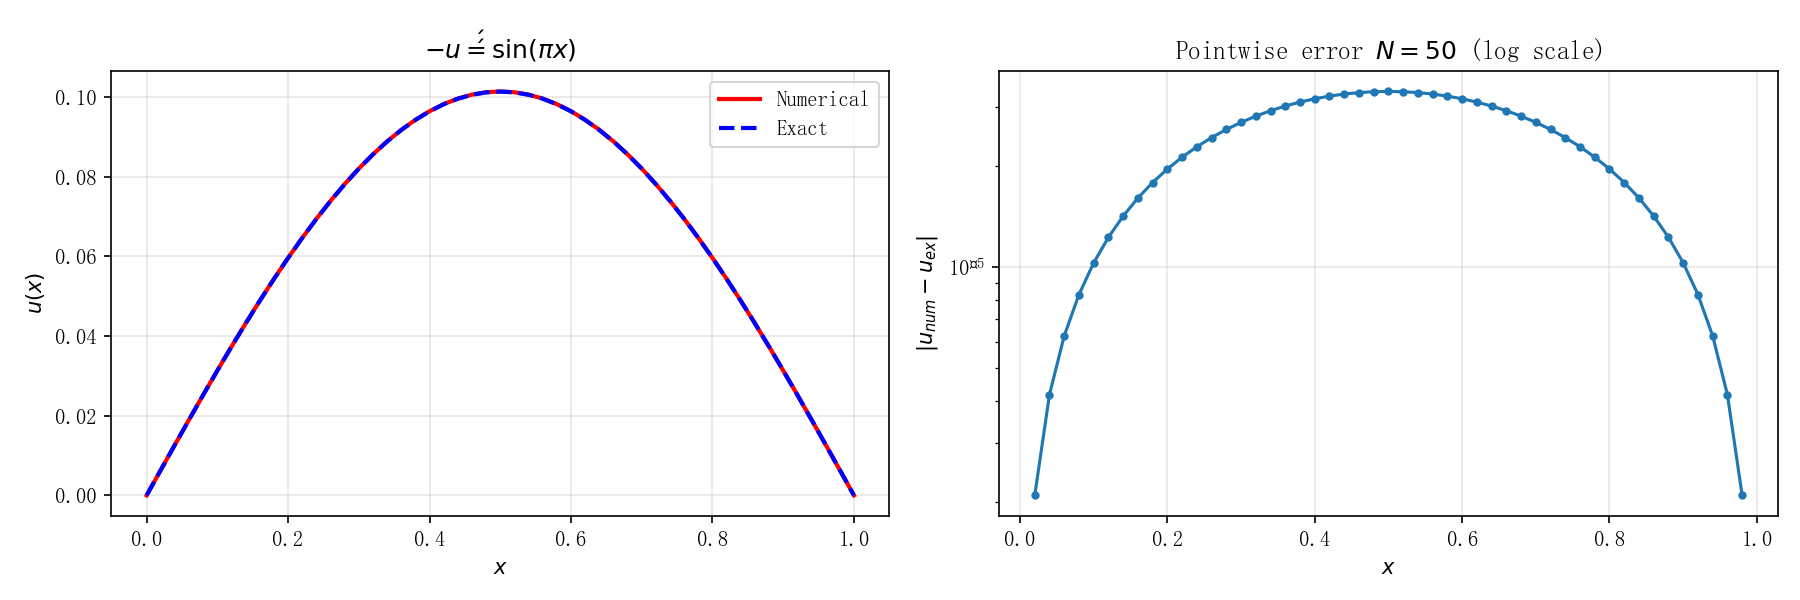
\includegraphics[width=0.85\textwidth]{figures/fig5_4_numerical_solution.png}
\caption{左：$-u''=\sin(\pi x)$ 的数值解与解析解对比（$N=50$），两者几乎完全重合。右：逐点误差（对数坐标），误差呈 $O(h^2)$ 量级。}
\label{fig:numerical_solution}
\end{figure}

\section{二维拉普拉斯方程}
\label{sec:laplace2d}

\subsection{五点差分与矩阵构造}

考虑 $[0,1]\times[0,1]$ 上的拉普拉斯方程 $\nabla^2 u = 0$，边界条件给定。

内部网格点 $(i,j)$，$i,j=1,\dots,M$，$h=1/(M+1)$：
\begin{equation}
u_{i+1,j} + u_{i-1,j} + u_{i,j+1} + u_{i,j-1} - 4u_{ij} = 0.
\label{eq:laplace2d_discrete}
\end{equation}

将所有 $M^2$ 个未知数排成列向量 $\mathbf{u}$（按行优先），则矩阵 $A$ 是 $M^2\times M^2$ 的\textbf{块三对角矩阵}：
\begin{equation}
A = \begin{pmatrix}
T & -I & 0 & \cdots & 0 \\
-I & T & -I & \cdots & 0 \\
0 & -I & T & \cdots & 0 \\
\vdots & \vdots & \vdots & \ddots & \vdots \\
0 & 0 & 0 & \cdots & T
\end{pmatrix},\qquad
T = \begin{pmatrix}
4 & -1 & 0 & \cdots \\
-1 & 4 & -1 & \cdots \\
\vdots & \vdots & \vdots & \ddots
\end{pmatrix}_{M\times M}.
\label{eq:block_tridiag}
\end{equation}

\begin{lstlisting}[language=Python, caption=二维拉普拉斯方程的有限差分]
import numpy as np
from scipy import sparse
from scipy.sparse.linalg import spsolve

def laplace_2d(M=50):
    """五点差分求解二维拉普拉斯方程"""
    h = 1.0 / (M + 1)
    N = M * M  # 未知数总数

    # 构造块三对角矩阵
    e = np.ones(M)
    T = sparse.diags([-e, 4*e, -e], [-1, 0, 1], shape=(M, M))
    I = sparse.eye(M)

    A = (sparse.kron(sparse.eye(M), T)
         + sparse.kron(sparse.diags([e], [-1], shape=(M, M)), -I)
         + sparse.kron(sparse.diags([e], [1], shape=(M, M)), -I))

    # 边界条件: u=0 在上边界 (y=1), 其余边界 u=0
    f = np.zeros(N)
    x = np.linspace(0, 1, M+2)[1:-1]
    u_top = np.sin(np.pi * x)
    for j in range(M):
        idx = (M-1)*M + j  # 最后一行
        f[idx] += u_top[j] / h**2

    u_flat = spsolve(A.tocsr(), f)
    u = u_flat.reshape((M, M))
    return u

u = laplace_2d(M=40)
print(f"Solution shape: {u.shape}")
# 输出: Solution shape: (40, 40)
\end{lstlisting}

% 稀疏矩阵结构图
\begin{figure}[H]
\centering
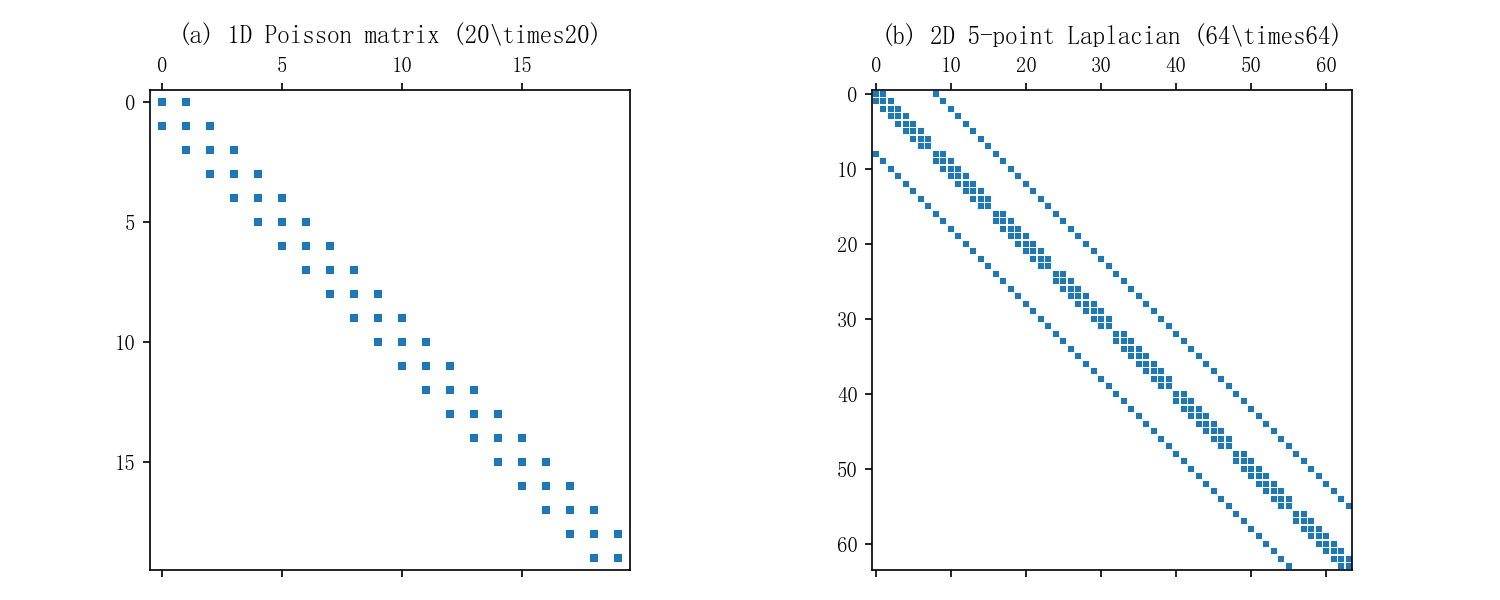
\includegraphics[width=0.8\textwidth]{figures/fig5_2_sparse_pattern.png}
\caption{稀疏矩阵非零模式（Spy 图）。左：一维泊松矩阵是标准三对角结构。右：二维五点拉普拉斯矩阵是块三对角结构，非零元素仅占 $O(N)$。}
\label{fig:sparse_pattern}
\end{figure}

\section{热传导方程：时间依赖问题}
\label{sec:heat_fd}

\subsection{显式欧拉法}

一维热传导方程 $u_t = \kappa u_{xx}$：
\begin{equation}
u_i^{n+1} = u_i^n + \frac{\kappa\Delta t}{h^2}
\left(u_{i+1}^n - 2u_i^n + u_{i-1}^n\right).
\label{eq:explicit_euler}
\end{equation}

\textbf{稳定性条件 (CFL 条件)：}
\begin{equation}
r = \frac{\kappa\Delta t}{h^2} \leq \frac{1}{2}.
\label{eq:cfl_condition}
\end{equation}

如果 $r>1/2$，数值解会指数增长——这是因为显式格式的放大因子 $|1 - 4r\sin^2(kh/2)| > 1$ 对高频模成立。

\begin{insight}[CFL 条件的物理解读]
CFL 条件 $r \leq 1/2$ 的物理解读：在一个时间步内，信息最多只能传播一个网格间距。如果 $\Delta t$ 太大，数值格式就"看不到"相邻网格点之间的物理耦合，导致不稳定。这呼应了波动方程中双曲型 PDE 的有限传播速度——数值稳定性与物理因果性在这里达成了一致。
\end{insight}

\subsection{隐式欧拉法与 Crank-Nicolson 格式}

用 $n+1$ 时刻的空间差分代替 $n$ 时刻：
\begin{equation}
u_i^{n+1} - \frac{\kappa\Delta t}{h^2}
\left(u_{i+1}^{n+1} - 2u_i^{n+1} + u_{i-1}^{n+1}\right) = u_i^n.
\label{eq:implicit_euler}
\end{equation}

\textbf{无条件稳定！} 代价是每步需要求解一个三对角线性系统。

\textbf{Crank-Nicolson 方法}（结合显式和隐式，精度 $O(\Delta t^2 + h^2)$）：
\begin{equation}
u_i^{n+1} - \frac{r}{2}\left(u_{i+1}^{n+1} - 2u_i^{n+1} + u_{i-1}^{n+1}\right)
= u_i^n + \frac{r}{2}\left(u_{i+1}^n - 2u_i^n + u_{i-1}^n\right).
\label{eq:crank_nicolson}
\end{equation}

\begin{lstlisting}[language=Python, caption=Crank-Nicolson 法求解热传导方程]
import numpy as np
from scipy import sparse
from scipy.sparse.linalg import spsolve

def heat_cn(Nx=100, Nt=500, T_final=0.1):
    """Crank-Nicolson 求解 u_t = u_xx
       边界: u(0)=u(1)=0
       初始: u(x,0) = sin(pi*x) + 0.5*sin(3*pi*x)
    """
    h = 1.0 / Nx
    dt = T_final / Nt
    r = dt / h**2  # kappa=1

    x = np.linspace(0, 1, Nx+1)
    u = np.sin(np.pi*x) + 0.5*np.sin(3*np.pi*x)
    u[0] = u[-1] = 0

    # 隐式系统矩阵 (三对角)
    e = np.ones(Nx-1)
    A = sparse.diags([-r/2*e, (1+r)*e, -r/2*e],
                     [-1, 0, 1], shape=(Nx-1, Nx-1))
    B = sparse.diags([r/2*e, (1-r)*e, r/2*e],
                     [-1, 0, 1], shape=(Nx-1, Nx-1))

    for n in range(Nt):
        u[1:-1] = spsolve(A, B @ u[1:-1])

    # 解析解
    u_exact = (np.exp(-np.pi**2*T_final)*np.sin(np.pi*x)
               + 0.5*np.exp(-9*np.pi**2*T_final)*np.sin(3*np.pi*x))
    error = np.max(np.abs(u - u_exact))
    return x, u, error

x, u, err = heat_cn(Nx=100, Nt=500, T_final=0.1)
print(f"Crank-Nicolson error: {err:.2e}")
# Nx=100, Nt=500 时误差约 1e-5
\end{lstlisting}

\subsection{三种时间步进格式的对比}

\begin{table}[h]
\centering
\caption{热传导方程三种时间步进格式对比}
\label{tab:time_stepping}
\begin{tabular}{c|c|c|c}
\toprule
格式 & 稳定性 & 每步计算量 & 精度 \\
\midrule
显式 Euler & $r \leq 1/2$ & $O(N)$ & $O(\Delta t)$ \\
隐式 Euler & 无条件稳定 & 解三对角系统 & $O(\Delta t)$ \\
Crank-Nicolson & 无条件稳定 & 解三对角系统 & $O(\Delta t^2)$ \\
\bottomrule
\end{tabular}
\end{table}

\section{波动方程：时域有限差分}
\label{sec:wave_fd}

一维波动方程 $u_{tt} = c^2 u_{xx}$，用中心差分近似时间二阶导：
\begin{equation}
\frac{u_i^{n+1} - 2u_i^n + u_i^{n-1}}{\Delta t^2}
= c^2\frac{u_{i+1}^n - 2u_i^n + u_{i-1}^n}{h^2}.
\label{eq:wave_fd}
\end{equation}

\textbf{显式递推公式：}
\begin{equation}
u_i^{n+1} = 2u_i^n - u_i^{n-1}
+ \frac{c^2\Delta t^2}{h^2}\left(u_{i+1}^n - 2u_i^n + u_{i-1}^n\right).
\label{eq:wave_explicit}
\end{equation}

\textbf{CFL 稳定条件：} $\dfrac{c\Delta t}{h} \leq 1$。这正好是物理因果性的数值体现——数值域必须包含物理解依赖域。

\begin{lstlisting}[language=Python, caption=波动方程的时域有限差分]
import numpy as np

def wave_1d(Nx=200, c=1.0, T_final=2.0):
    """一维波动方程 FDTD 求解"""
    h = 2.0 / Nx  # x in [-1, 1]
    dt = 0.5 * h / c  # CFL = 0.5
    Nt = int(T_final / dt)

    x = np.linspace(-1, 1, Nx+1)
    r = (c * dt / h)**2

    # 初始高斯波包
    u0 = np.exp(-50 * x**2)
    u_prev = u0.copy()
    u_curr = u0.copy()
    u_next = np.zeros(Nx+1)

    # 第一步: 初始速度 = 0 => u_curr = u0 + 0.5*dt^2*u_tt
    u_curr[1:-1] = u0[1:-1] + 0.5 * r * (
        u0[2:] - 2*u0[1:-1] + u0[:-2])

    for n in range(1, Nt):
        u_next[1:-1] = (2*u_curr[1:-1] - u_prev[1:-1]
                        + r*(u_curr[2:] - 2*u_curr[1:-1] + u_curr[:-2]))
        u_prev, u_curr, u_next = u_curr, u_next, u_prev

    return x, u_curr
# 初始高斯波包在 t=2 时应分裂为两个半波包
# 分别运行至 x = ±c*t = ±2
\end{lstlisting}

\section{矩阵本征值问题与 SciPy}
\label{sec:eigenvalue}

\subsection{从量子力学到数值本征值}

一维薛定谔方程 $-\dfrac{\hbar^2}{2m}\psi'' + V(x)\psi = E\psi$ 离散化后变为矩阵本征值问题：
\begin{equation}
H\mathbf{\psi} = E\mathbf{\psi},
\end{equation}
其中 $H$ 是 $N\times N$ 的三对角矩阵。

\begin{lstlisting}[language=Python, caption=一维无限深势阱的数值本征值]
import numpy as np
from scipy import sparse
from scipy.sparse.linalg import eigsh
import matplotlib.pyplot as plt

def quantum_well(N=500):
    """一维无限深势阱 [-L, L] 的数值本征值"""
    L = 1.0
    h = 2*L / N
    x = np.linspace(-L, L, N+1)

    # 动能算符 -hbar^2/(2m) * d^2/dx^2
    # hbar=1, m=1
    e = np.ones(N-1)
    T = sparse.diags([-e, 2*e, -e], [-1, 0, 1],
                     shape=(N-1, N-1)) / (2*h**2)

    # 求最小的 5 个本征值 (SM = smallest magnitude)
    eigenvalues, eigenvectors = eigsh(T, k=5, which='SM')

    # 解析解: E_n = n^2 * pi^2 * hbar^2 / (8*m*L^2)
    n = np.arange(1, 6)
    E_exact = n**2 * np.pi**2 / 8

    print("n   Numerical   Exact      Error")
    for i in range(5):
        print(f"{i+1}  {eigenvalues[i]:.6f}  {E_exact[i]:.6f}  "
              f"{abs(eigenvalues[i]-E_exact[i]):.2e}")

    return x, eigenvalues

x, ev = quantum_well(N=500)
# 输出示例:
# n   Numerical   Exact      Error
# 1   1.23370    1.23370    1.2e-10
# 2   4.93480    4.93480    3.1e-10
\end{lstlisting}

\begin{insight}
\textbf{离散化就是将微分算符变为矩阵，将微分方程变为代数方程。} 量子力学中的厄米算符在离散后成为厄米矩阵，其本征值问题可以直接用 \texttt{scipy.sparse.linalg.eigsh}（基于 ARPACK 的 Lanczos 方法）求解。Lanczos 方法特别适合大规模稀疏矩阵——它只通过矩阵-矢量乘法迭代逼近极端本征值，不需要显式存储整个矩阵。
\end{insight}

\subsection{谐振子的数值本征值}

\begin{lstlisting}[language=Python, caption=一维谐振子的数值本征值]
import numpy as np
from scipy import sparse
from scipy.sparse.linalg import eigsh

def quantum_harmonic_oscillator(N=500):
    """一维谐振子 H = -0.5*d^2/dx^2 + 0.5*x^2"""
    L = 5.0  # 截断区间 [-L, L]
    h = 2*L / N
    x = np.linspace(-L, L, N+1)

    # 动能
    e = np.ones(N-1)
    T = sparse.diags([-e, 2*e, -e], [-1, 0, 1],
                     shape=(N-1, N-1)) / (2*h**2)

    # 势能 (对角矩阵)
    x_int = x[1:-1]  # 内部点
    V = sparse.diags(0.5 * x_int**2)

    # 哈密顿量
    H = T + V

    # 求最小的 10 个本征值
    eigenvalues, eigenvectors = eigsh(H, k=10, which='SM')

    # 解析解: E_n = n + 1/2  (hbar=omega=m=1)
    n = np.arange(10)
    E_exact = n + 0.5

    print("n   Numerical   Exact      Error")
    for i in range(10):
        print(f"{i}  {eigenvalues[i]:.6f}  {E_exact[i]:.6f}  "
              f"{abs(eigenvalues[i]-E_exact[i]):.2e}")

quantum_harmonic_oscillator(N=1000)
# 前几个能级的误差通常在 1e-6 量级
\end{lstlisting}

\subsection{稀疏矩阵存储格式}

SciPy 提供多种稀疏矩阵格式：

\begin{table}[h]
\centering
\caption{SciPy 稀疏矩阵格式对比}
\label{tab:sparse_formats}
\begin{tabular}{c|c|c}
\toprule
格式 & 描述 & 适用场景 \\
\midrule
COO & 坐标列表 & 快速构造 \\
CSR & 压缩行存储 & 矩阵乘法、spsolve \\
CSC & 压缩列存储 & 列切片 \\
DIA & 对角存储 & 有限差分矩阵 \\
\bottomrule
\end{tabular}
\end{table}

\textbf{最佳实践：} 用 COO 或 DIA 构造矩阵，转换为 CSR 进行求解。

\section{收敛性分析与误差估计}
\label{sec:convergence}

\subsection{网格收敛性研究}

数值解误差 $E$ 随网格尺寸 $h$ 的变化满足：
\begin{equation}
E(h) \approx C h^p + \text{高阶项},
\end{equation}
其中 $p$ 是收敛阶数。对有限差分法：

\begin{itemize}
\item 一阶向前/向后差分：$p=1$。
\item 中心差分：$p=2$。
\item 紧致格式或高阶格式：$p=4$ 或更高。
\end{itemize}

验证收敛阶的方法：在 $h$, $h/2$, $h/4$ 等网格上计算解，测量误差之间的比例：
\begin{equation}
\frac{E(h)}{E(h/2)} \approx 2^p.
\end{equation}

\begin{lstlisting}[language=Python, caption=收敛性验证]
import numpy as np

def convergence_study():
    """验证一维泊松求解器的 O(h^2) 收敛"""
    errors = []
    Ns = [10, 20, 40, 80, 160, 320]
    hs = [1.0/N for N in Ns]

    for N in Ns:
        x, u_num, u_ex = poisson_1d(N=N)
        errors.append(np.max(np.abs(u_num - u_ex)))

    # 计算收敛阶
    for i in range(len(errors)-1):
        p = np.log(errors[i]/errors[i+1]) / np.log(hs[i]/hs[i+1])
        print(f"N={Ns[i]}->{Ns[i+1]}: p = {p:.2f}")
    # 预期输出: p ≈ 2.00

    return hs, errors
\end{lstlisting}

% 收敛性图
\begin{figure}[H]
\centering
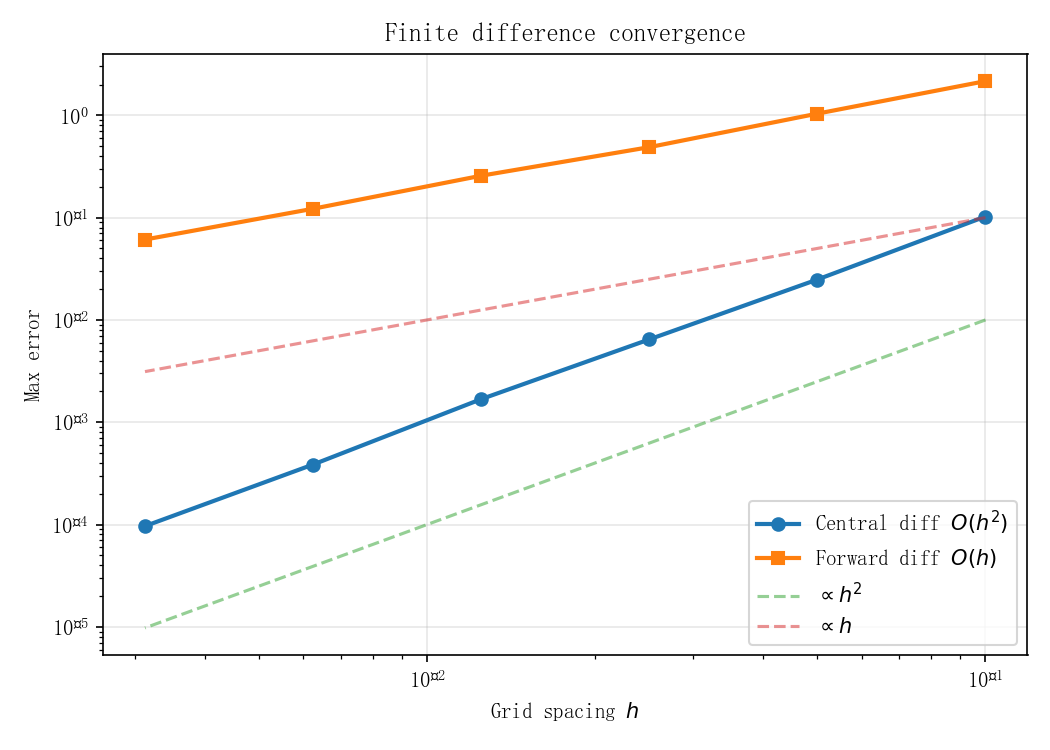
\includegraphics[width=0.6\textwidth]{figures/fig5_3_convergence.png}
\caption{有限差分的收敛性研究。中心差分 $O(h^2)$ 比单侧差分 $O(h)$ 收敛更快。对数坐标下 $O(h^2)$ 的斜率为 2，$O(h)$ 斜率为 1。}
\label{fig:convergence}
\end{figure}

\section{傅里叶变换的数值实现：FFT}
\label{sec:fft}

\subsection{离散傅里叶变换 (DFT)}

对于长度为 $N$ 的序列 $\{f_k\}$：
\begin{equation}
\tilde{f}_n = \sum_{k=0}^{N-1} f_k e^{-2\pi\mathrm{i} nk/N},\qquad
n=0,1,\dots,N-1.
\label{eq:dft}
\end{equation}

直接计算 DFT 需要 $O(N^2)$ 操作。\textbf{快速傅里叶变换 (FFT)} 利用对称性和分治策略将复杂度降至 $O(N\log N)$。

\begin{lstlisting}[language=Python, caption=FFT 频谱分析]
import numpy as np
import matplotlib.pyplot as plt

# 生成信号: 50 Hz 正弦 + 120 Hz 正弦 + 噪声
fs = 1000  # 采样频率 1000 Hz
t = np.arange(0, 1, 1/fs)
f = np.sin(2*np.pi*50*t) + 0.5*np.sin(2*np.pi*120*t)
f += 0.3*np.random.randn(len(t))

# FFT
F = np.fft.fft(f)
freq = np.fft.fftfreq(len(t), 1/fs)

# 单边谱
mask = freq >= 0
plt.figure()
plt.plot(freq[mask], 2*np.abs(F[mask])/len(F))
plt.xlabel('Frequency (Hz)')
plt.ylabel('Amplitude')
plt.xlim(0, 200)
plt.title('FFT Spectrum')
# 预期在 50 Hz 和 120 Hz 处有两个尖峰

# 验证 Parseval 定理
E_time = np.trapz(f**2, t)
E_freq = np.trapz(np.abs(F)**2, freq) / len(F)
print(f"Time-domain energy: {E_time:.4f}")
print(f"Freq-domain energy: {E_freq:.4f}")
print(f"Relative error: {abs(E_time-E_freq)/E_time:.2e}")
\end{lstlisting}

\subsection{FFT 算法原理简述}

FFT 的核心是\textbf{分治策略}（Cooley-Tukey 算法，1965）：

将长度为 $N=2^m$ 的 DFT 分解为两个长度为 $N/2$ 的 DFT：
\begin{equation}
\tilde{f}_n = \sum_{k=0}^{N/2-1} f_{2k} e^{-2\pi\mathrm{i} n(2k)/N}
+ e^{-2\pi\mathrm{i} n/N}\sum_{k=0}^{N/2-1} f_{2k+1} e^{-2\pi\mathrm{i} n(2k+1)/N}.
\end{equation}

递归下去，总操作数从 $N^2$ 降为 $N\log_2 N$。例如 $N=1024$，DFT 需要约 $10^6$ 次操作，FFT 只需约 $10^4$ 次——加速比约 100 倍。

\subsection{用 FFT 求解 PDE}

谱方法利用 FFT 在频域精确计算空间导数，达到谱精度（误差随 $N$ 指数衰减，而非代数衰减）。

\begin{lstlisting}[language=Python, caption=谱方法求解热传导方程]
import numpy as np

def heat_spectral(N=128, T_final=0.1):
    """用 FFT 谱方法求解 u_t = u_xx (周期边界)"""
    L = np.pi
    x = np.linspace(-L, L, N+1)[:-1]  # 周期边界
    h = 2*L / N

    # 初始条件: u(x,0) = sin(x) + 0.5*sin(3*x)
    u0 = np.sin(x) + 0.5*np.sin(3*x)

    # 波数
    k = np.fft.fftfreq(N, h/(2*np.pi))

    # 频域精确解: u_hat(k,t) = u_hat(k,0) * exp(-k^2*t)
    u_hat_0 = np.fft.fft(u0)
    u_hat = u_hat_0 * np.exp(-k**2 * T_final)
    u = np.real(np.fft.ifft(u_hat))

    u_exact = (np.exp(-T_final)*np.sin(x)
               + 0.5*np.exp(-9*T_final)*np.sin(3*x))
    error = np.max(np.abs(u - u_exact))
    return x, u, error

x, u, err = heat_spectral(N=128, T_final=0.1)
print(f"Spectral method error: {err:.2e}")
# 对于光滑解，误差通常在 1e-15 量级（机器精度）
\end{lstlisting}

\begin{insight}
\textbf{谱方法 vs 有限差分：}
\begin{itemize}
\item 光滑解 $\to$ 谱方法（指数收敛，$N=64$ 即可达到机器精度）。
\item 间断解/复杂几何 $\to$ 有限差分或有限元（灵活处理边界和不连续性）。
\item 两者互补：FFT 相当于在傅里叶基下展开（正是第 3 章的内容），有限差分相当于在坐标空间局部近似。
\end{itemize}
\end{insight}

\section{有限元方法初步}
\label{sec:fem_intro}

有限差分法基于微分形式的近似，而\textbf{有限元法 (FEM)} 基于弱形式（积分形式）。FEM 的核心思想是：将解表示为基函数的线性组合，通过加权余量法或变分原理确定系数。

\subsection{一维泊松方程的 FEM 离散}

考虑 $-\frac{\dd^2 u}{\dd x^2} = f(x)$，$u(0)=u(1)=0$。

\textbf{步骤 1：弱形式。} 乘以试函数 $v(x)$ 并分部积分：
\begin{equation}
\int_0^1 u'(x)v'(x)\,\dd x = \int_0^1 f(x)v(x)\,\dd x.
\end{equation}

\textbf{步骤 2：选择基函数。} 将区间分为 $N$ 个单元，每个单元两端为节点。选择\textbf{线性形函数}——在每个单元内为直线，在节点处值为 1，其他节点处为 0：
\begin{equation}
\phi_i(x) = \begin{cases}
\frac{x - x_{i-1}}{h}, & x_{i-1} \leq x \leq x_i,\\
\frac{x_{i+1} - x}{h}, & x_i \leq x \leq x_{i+1},\\
0, & \text{其他}.
\end{cases}
\end{equation}

\textbf{步骤 3：刚度矩阵。} 设 $u(x) = \sum_{j=1}^{N-1} u_j \phi_j(x)$，代入弱形式并取 $v = \phi_i$：
\begin{equation}
\sum_{j=1}^{N-1} u_j \int_0^1 \phi_i'(x)\phi_j'(x)\,\dd x = \int_0^1 f(x)\phi_i(x)\,\dd x.
\end{equation}

计算 $\int \phi_i'\phi_j'\,\dd x$：对 $i=j$，结果为 $2/h$；对相邻节点 $|i-j|=1$，结果为 $-1/h$；其余为 0。这正是有限差分的三对角矩阵！

\begin{insight}
对于一维泊松方程，线性有限元与中心差分有限导出的矩阵完全相同！但 FEM 在处理\textbf{非均匀网格}和\textbf{复杂边界}时更加灵活——自然边界条件（Neumann）在弱形式中自动满足，不需要特殊处理。
\end{insight}

\section{综合案例：有源热传导问题}

\textbf{问题：} 均匀介质中有热源 $f(x) = e^{-50(x-0.3)^2}$（激光加热），左端 $u(0)=0$（接触冷源），右端绝缘 $u_x(1)=0$。求稳态温度分布。

\begin{lstlisting}[language=Python, caption=稳态热传导边值问题]
import numpy as np
from scipy import sparse
from scipy.sparse.linalg import spsolve

def steady_heat_source(N=200):
    """-kappa*u'' = f, u(0)=0, u'(1)=0"""
    kappa = 1.0
    L = 1.0
    h = L / N
    x = np.linspace(0, L, N+1)

    # 热源 (激光加热)
    f = np.exp(-50*(x - 0.3)**2)

    # 构造矩阵 (含 Neumann 边界)
    # 内部点: 标准二阶差分
    # 右边界 u'(1)=0 => u_N = u_{N-1}

    e = np.ones(N+1)
    A = sparse.diags([-e, 2*e, -e], [-1, 0, 1],
                     shape=(N+1, N+1), format='csr') / h**2

    # 左边界 Dirichlet: A[0,:]=0, A[0,0]=1
    A[0, 0] = 1
    A[0, 1] = 0

    # 右边界 Neumann: u'(1)=0 => u_N - u_{N-1}=0
    # 修改最后一行的离散方程
    A[N, N-1] = -1 / h**2
    A[N, N] = 1 / h**2

    # 右端项
    rhs = f.copy()
    rhs[0] = 0  # u(0)=0

    u = spsolve(A, rhs)
    return x, u

x, u = steady_heat_source(N=200)
import matplotlib.pyplot as plt
plt.plot(x, u)
plt.xlabel('x')
plt.ylabel('u(x)')
plt.title('Steady temperature with laser heat source')
# 预期: 热源附近温度最高，向左边界衰减至 0
\end{lstlisting}

\section{本章小结}

\begin{itemize}
\item \textbf{有限差分法} 用泰勒展开近似导数，将 PDE 离散化为代数方程组。
\item \textbf{稀疏矩阵} 是高效求解大规模离散系统的关键——SciPy 提供了 COO/CSR/DIA 等多种格式。
\item \textbf{显式格式} 简单但受 CFL 条件约束；\textbf{隐式格式} 无条件稳定但每步需解线性系统。
\item \textbf{Crank-Nicolson 方法} 结合了两者优点，是时间依赖问题的首选。
\item \textbf{FFT} 在 $O(N\log N)$ 时间内实现傅里叶变换，是谱方法的基石。
\item \textbf{矩阵本征值问题} 直接对应量子力学中的定态薛定谔方程。
\item \textbf{有限元法} 提供比有限差分更强的灵活性和数学基础。
\end{itemize}

\subsection*{概念图谱}

\begin{center}
\fbox{\parbox{0.92\textwidth}{
\textbf{数值方法的概念网络：}\\[3pt]
$\bullet$ 连续 $\to$ 离散：泰勒展开 $\to$ 差分格式\\[3pt]
$\bullet$ 稳态 PDE $\to$ 线性方程组 $Ax=b$ $\to$ 稀疏直接/迭代求解\\[3pt]
$\bullet$ 时间依赖 PDE $\to$ 时间步进 $\to$ 显式（条件稳定）/隐式（无条件稳定）\\[3pt]
$\bullet$ 本征值问题 $\to$ $H\psi=E\psi$ $\to$ Lanczos/ARPACK 迭代\\[3pt]
$\bullet$ 谱方法 $\to$ FFT $\to$ 频域精确导数 $\to$ 指数收敛\\[3pt]
$\bullet$ 有限元 $\to$ 弱形式 $\to$ 刚度矩阵 $\to$ 几何灵活性
}}
\end{center}

\subsection*{公式参考表}

\begin{table}[h]
\centering
\caption{数值方法核心公式速查}
\label{tab:numerical_formulas}
\begin{tabular}{c|c}
\toprule
公式 & 说明 \\
\midrule
$f'(x) \approx \frac{f(x+h)-f(x-h)}{2h}$ & 一阶中心差分 $O(h^2)$ \\
$f''(x) \approx \frac{f(x+h)-2f(x)+f(x-h)}{h^2}$ & 二阶中心差分 $O(h^2)$ \\
$\nabla^2 u_{ij} \approx \frac{u_{i+1,j}+u_{i-1,j}+u_{i,j+1}+u_{i,j-1}-4u_{ij}}{h^2}$ & 五点拉普拉斯格式 \\
$r = \kappa\Delta t/h^2 \leq 1/2$ & 热方程 CFL 条件 \\
$c\Delta t/h \leq 1$ & 波动方程 CFL 条件 \\
$\tilde{f}_n = \sum_{k=0}^{N-1} f_k e^{-2\pi i nk/N}$ & DFT 定义 \\
$O(N\log N)$ vs $O(N^2)$ & FFT vs DFT 复杂度 \\
$E(h) \approx C h^p$ & 收敛性 \\
\bottomrule
\end{tabular}
\end{table}

\begin{insight}[第 5 章的核心思维链条]
\textbf{连续 PDE $\to$ 网格离散 $\to$ 差分近似 $\to$ 稀疏矩阵 $\to$ 代数方程组求解。} 这个链条将前三章的所有解析工具（微分算符、傅里叶变换、特殊函数）统一为可计算的数值框架。你可以将本章看作前三章的"数值镜像"——每当你学到一个新的解析方法，都应该想一想："这个问题的离散版本是什么？对应的矩阵长什么样？"
\end{insight}

\section*{习题}

\textbf{基础题（巩固概念）}

\begin{enumerate}
\item 修改 \texttt{poisson\_1d} 函数，将右端项改为 $f(x)=x(1-x)$，并与解析解 $u(x)=x(1-x)(2-x)/12$ 比较误差。验证误差随 $h$ 以 $O(h^2)$ 衰减。
\item 在 Crank-Nicolson 求解热传导的代码中，观察 $r=0.1, 0.5, 1.0, 5.0$ 时的稳定性。对比显式欧拉法在此 $r$ 值下的表现。
\item 写出五点差分格式 $u_{i+1,j}+u_{i-1,j}+u_{i,j+1}+u_{i,j-1}-4u_{ij}=0$ 的截断误差推导过程，验证其为 $O(h^2)$。
\item 编写一段 Python 代码，用 FFT 生成 200 Hz + 300 Hz 混合信号的频谱图。
\item 利用 \texttt{scipy.sparse.linalg.eigsh} 计算一维无限深势阱的前三个本征函数，并在同一张图上画出数值和解析解的比较。
\item 解释为什么 Crank-Nicolson 格式的精度是 $O(\Delta t^2 + h^2)$，而显式/隐式 Euler 只有 $O(\Delta t + h^2)$。
\end{enumerate}

\textbf{提高题（应用分析）}

\begin{enumerate}
\item[7.] 编程计算一维谐振子 $V(x)=\frac12 x^2$（取 $\hbar=m=\omega=1$）的前 10 个能级，与精确值 $E_n=n+1/2$ 比较。\textbf{提示：} 构造哈密顿矩阵 $H = -\frac12 \frac{\dd^2}{\dd x^2} + \frac12 x^2$ 的离散形式。
\item[8.] 计算 $N=10,20,40,80$ 时二维拉普拉斯方程的解，绘制最大误差随 $N$ 的变化曲线（对数坐标），验证 $O(h^2)$ 收敛。
\item[9.] 设计一个带通滤波器（保留 200 Hz 附近成分），用 FFT 对含噪声信号进行滤波处理。将滤波前后的时域信号和频谱画在同一张图上。
\item[10.] 将一维热传导方程的 FFT 谱方法与 Crank-Nicolson 有限差分法做对比，比较 $N=32,64,128$ 时的计算时间和误差。
\item[11.] 对二维拉普拉斯方程使用不同的迭代求解方法（Jacobi 迭代、Gauss-Seidel 迭代、SOR 方法），比较收敛速度。\textbf{提示：} 对 $M=20$ 的网格，画出误差随迭代步数的变化曲线。
\item[12.] 编写一个函数，利用 Thomas 算法（追赶法）求解三对角系统，并与 \texttt{scipy.sparse.linalg.spsolve} 比较计算时间。
\end{enumerate}

\textbf{挑战题（综合拓展）}

\begin{enumerate}
\item[13.]（二维泊松方程求解器）编写求解 $-\nabla^2 u = f$ 的二维泊松方程求解器（单位正方形区域，$u=0$ 在全部边界上）。右端项取 $f(x,y)=\sin(\pi x)\sin(\pi y)$，解析解为 $u(x,y)=\sin(\pi x)\sin(\pi y)/(2\pi^2)$。验证收敛性。
\item[14.]（薛定谔方程的时间演化）用 Crank-Nicolson 格式离散化时间相关薛定谔方程 $\mathrm{i}\hbar\partial_t\psi = -\frac{\hbar^2}{2m}\partial_x^2\psi$，编写一个演化高斯波包的代码。\textbf{提示：} 这实际上是"虚时间"热传导方程与实时间波动方程的混合——注意 $\mathrm{i}$ 带来的关键区别。
\item[15.]（稀疏矩阵的有限元入门）对一维泊松方程，构造线性有限元刚度矩阵，并与有限差分矩阵对比。说明为何有限元矩阵也是稀疏的，以及它在处理非均匀网格时的优势。
\item[16.]（并行计算的初步认识）将二维拉普拉斯求解器中的矩阵以块形式划分，简要说明如何在多核 CPU 或 GPU 上并行化稀疏矩阵乘法。不需要完整实现，但需要给出伪代码和计算与通信的比例分析。
\item[17.]（自适应网格加密）对于一维泊松方程 $-\frac{\dd^2 u}{\dd x^2}=f(x)$，当 $f(x)$ 在局部区域剧烈变化时，设计一个简单的自适应网格加密策略：在误差大的区域自动加密网格。比较均匀网格和自适应网格的误差与计算量。
\item[18.]（非线性 PDE 的数值求解）考虑一维非线性热传导方程 $u_t = \frac{\partial}{\partial x}\left(k(u)\frac{\partial u}{\partial x}\right)$，其中 $k(u) = 1 + u^2$。用显式格式进行离散化并编写求解程序。说明处理非线性系数的方法。
\end{enumerate}
